\documentclass{article}

\usepackage[utf8]{inputenc}

\usepackage{amsmath, bm}
\usepackage{graphicx}
\usepackage{amssymb}
\usepackage{float}
\usepackage{caption}
\usepackage{subcaption}
\usepackage{hyperref}
\usepackage{tikz}
\usepackage{layout}
\usepackage{booktabs}

\usepackage[margin=1in]{geometry}
\usepackage{listings}
\usepackage{xcolor}
\usepackage{color, colortbl}
\usepackage{textgreek}
\usepackage{mathrsfs}
\usepackage{savetrees}

\usetikzlibrary{calc}
\usetikzlibrary{angles,quotes} % for pic
\usetikzlibrary{patterns,snakes}
\usetikzlibrary{arrows}
\tikzset{>=latex} % for LaTeX arrow head

\setlength{\parskip}{\baselineskip}%
\setlength{\parindent}{0pt}%
\linespread{0.9}


\definecolor{codegreen}{rgb}{0,0.6,0}
\definecolor{codegray}{rgb}{0.5,0.5,0.5}
\definecolor{codepurple}{rgb}{0.58,0,0.82}
\definecolor{backcolour}{rgb}{0.95,0.95,0.92}

\lstdefinestyle{mystyle}{
    backgroundcolor=\color{backcolour},   
    commentstyle=\color{codegreen},
    keywordstyle=\color{magenta},
    numberstyle=\tiny\color{codegray},
    stringstyle=\color{codepurple},
    basicstyle=\ttfamily\footnotesize,
    breakatwhitespace=false,         
    breaklines=true,                 
    captionpos=b,                    
    keepspaces=true,                 
    numbers=left,                    
    numbersep=5pt,                  
    showspaces=false,                
    showstringspaces=false,
    showtabs=false,                  
    tabsize=2
}

\lstset{style=mystyle}



\begin{document}

\title{Computational Fluid Dynamics \\
    \large Interim Report}
\author{lwp26}
\date{October 2024}
\maketitle 

\iffalse
\begin{abstract}
    \centering

\end{abstract}
\fi

%-----------------------------------------------------------------------------------------
\section{Introduction}
%-----------------------------------------------------------------------------------------

\subsection{Purpose}


\subsection{Results}

\begin{table}[h!]
    \centering
    \begin{tabular}{lcc}
        \toprule
        \textbf{Configuration} & \textbf{Run Time Normalised, Averaged } & \textbf{Variation Coefficient Run Time} \\
        \midrule
        Debug & 6.83 & 0.021 \\
        Release O2 & 1.05 & 0.018 \\
        Release O2, QxHost & 1.69 & 0.049 \\
        Release O2, Qparallel & 2.66 & 0.087 \\
        Release O2, fp:fast & 1.01 & 0.036 \\
        Release O3 & 1.09 & 0.016 \\
        Release O3, fp:fast & 1.00 & 0.010 \\
        Release O2 & 1.03 & 0.019 \\
        \bottomrule
    \end{tabular}
    \caption{Standard bump case run times for various compiler flags, normalised by the minimum averaged time. The average and deviation were found over three runs at a low $CFL$ such that 20,000 iterations were performed.}
    \label{tab:performance}
\end{table}

\begin{figure}
    \centering
    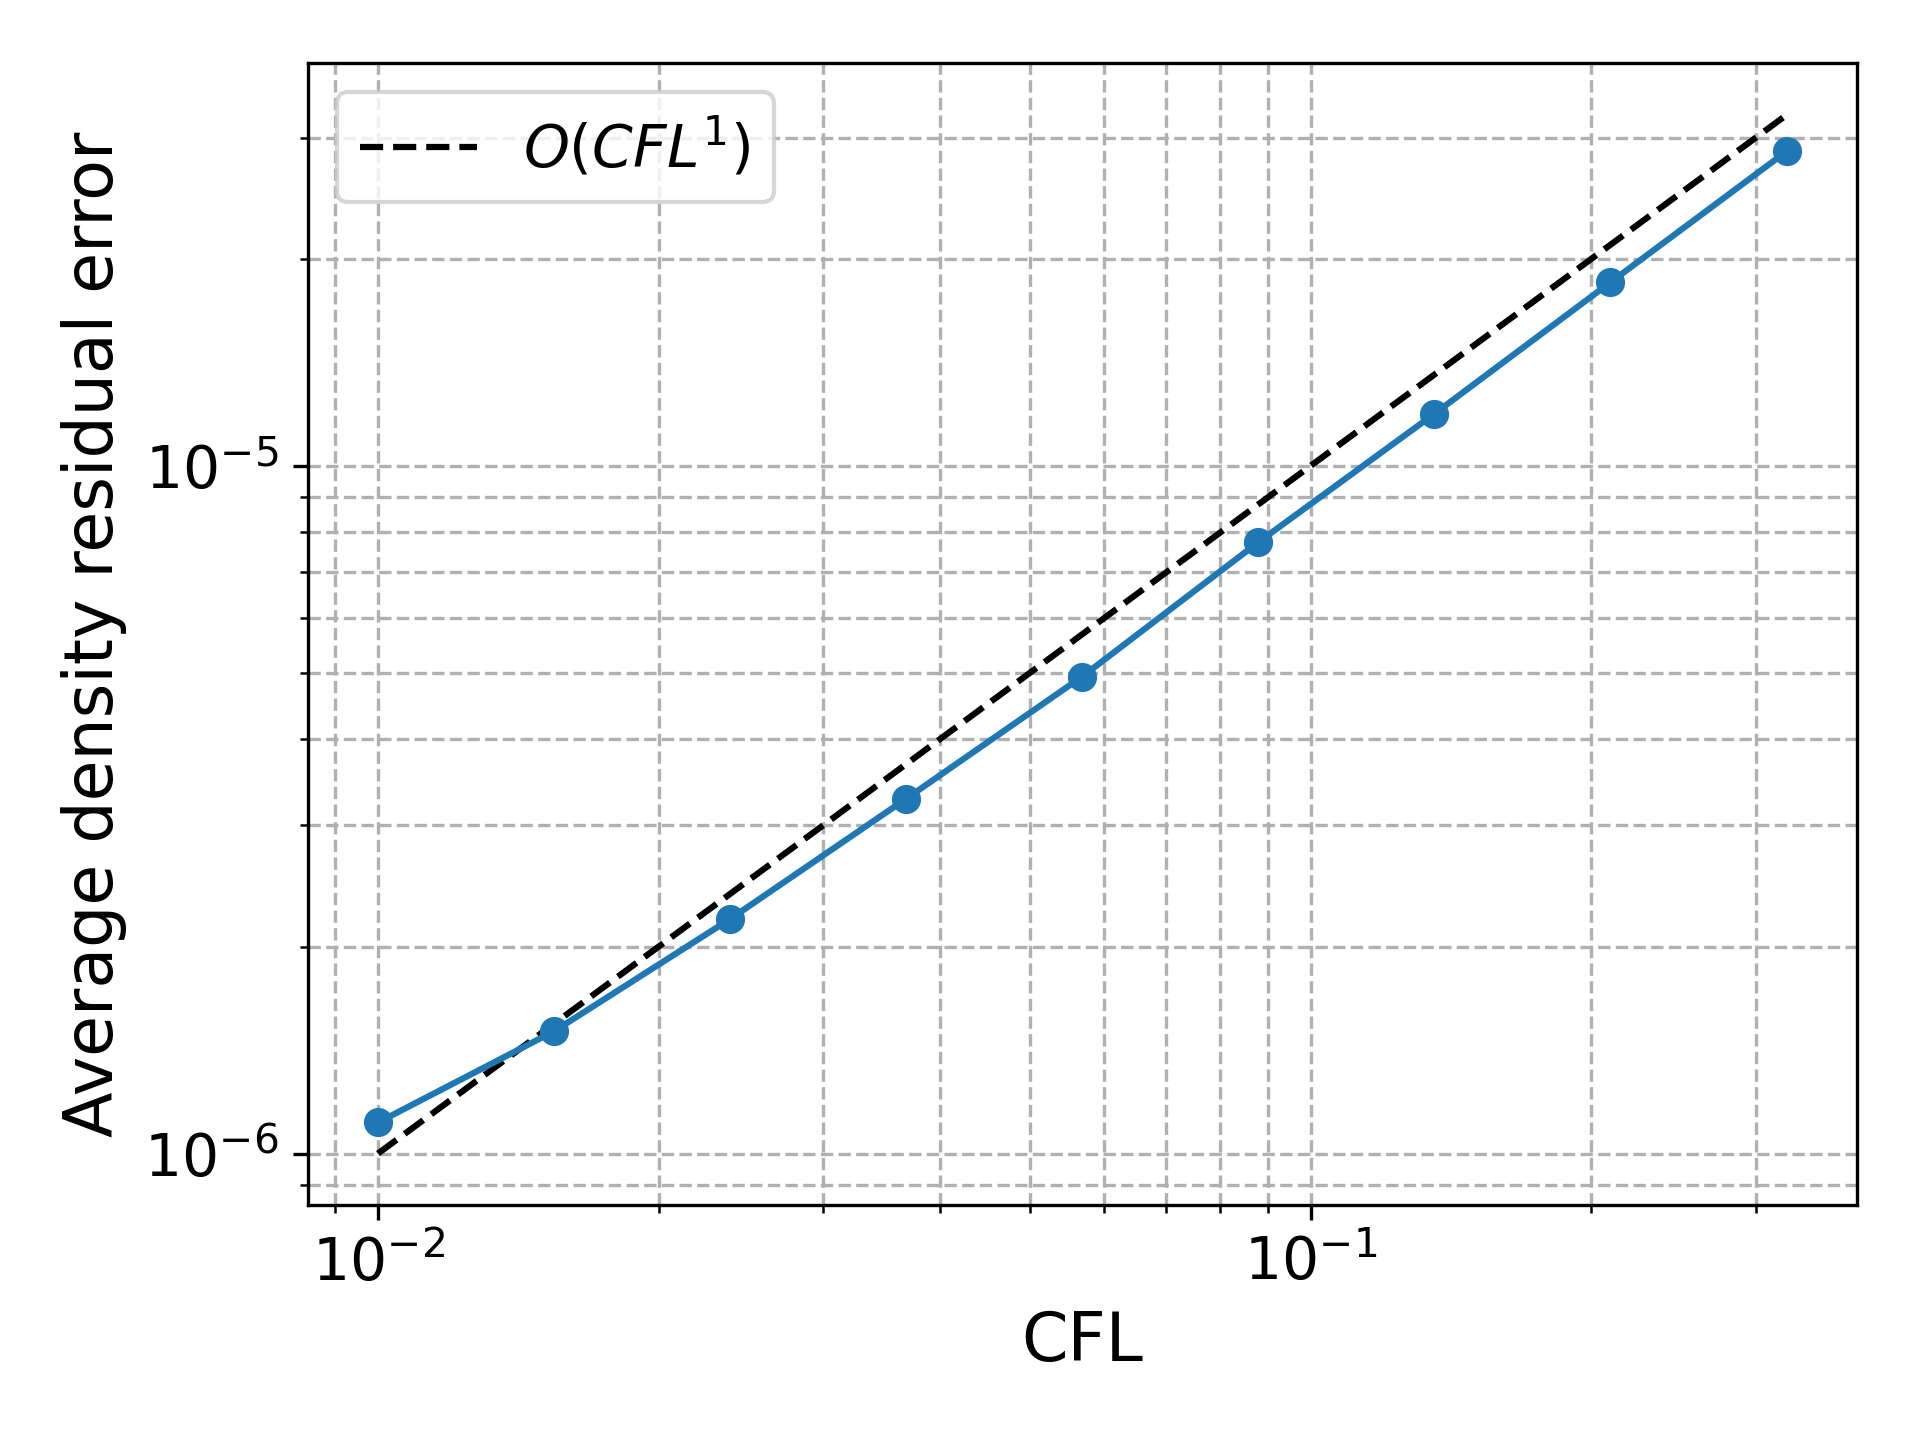
\includegraphics[width=0.8\textwidth]{figures/bump_d_avg_cfl.png}
    \caption{}
    \label{fig:bump_d_avg_cfl}
\end{figure}

\begin{figure}
    \centering
    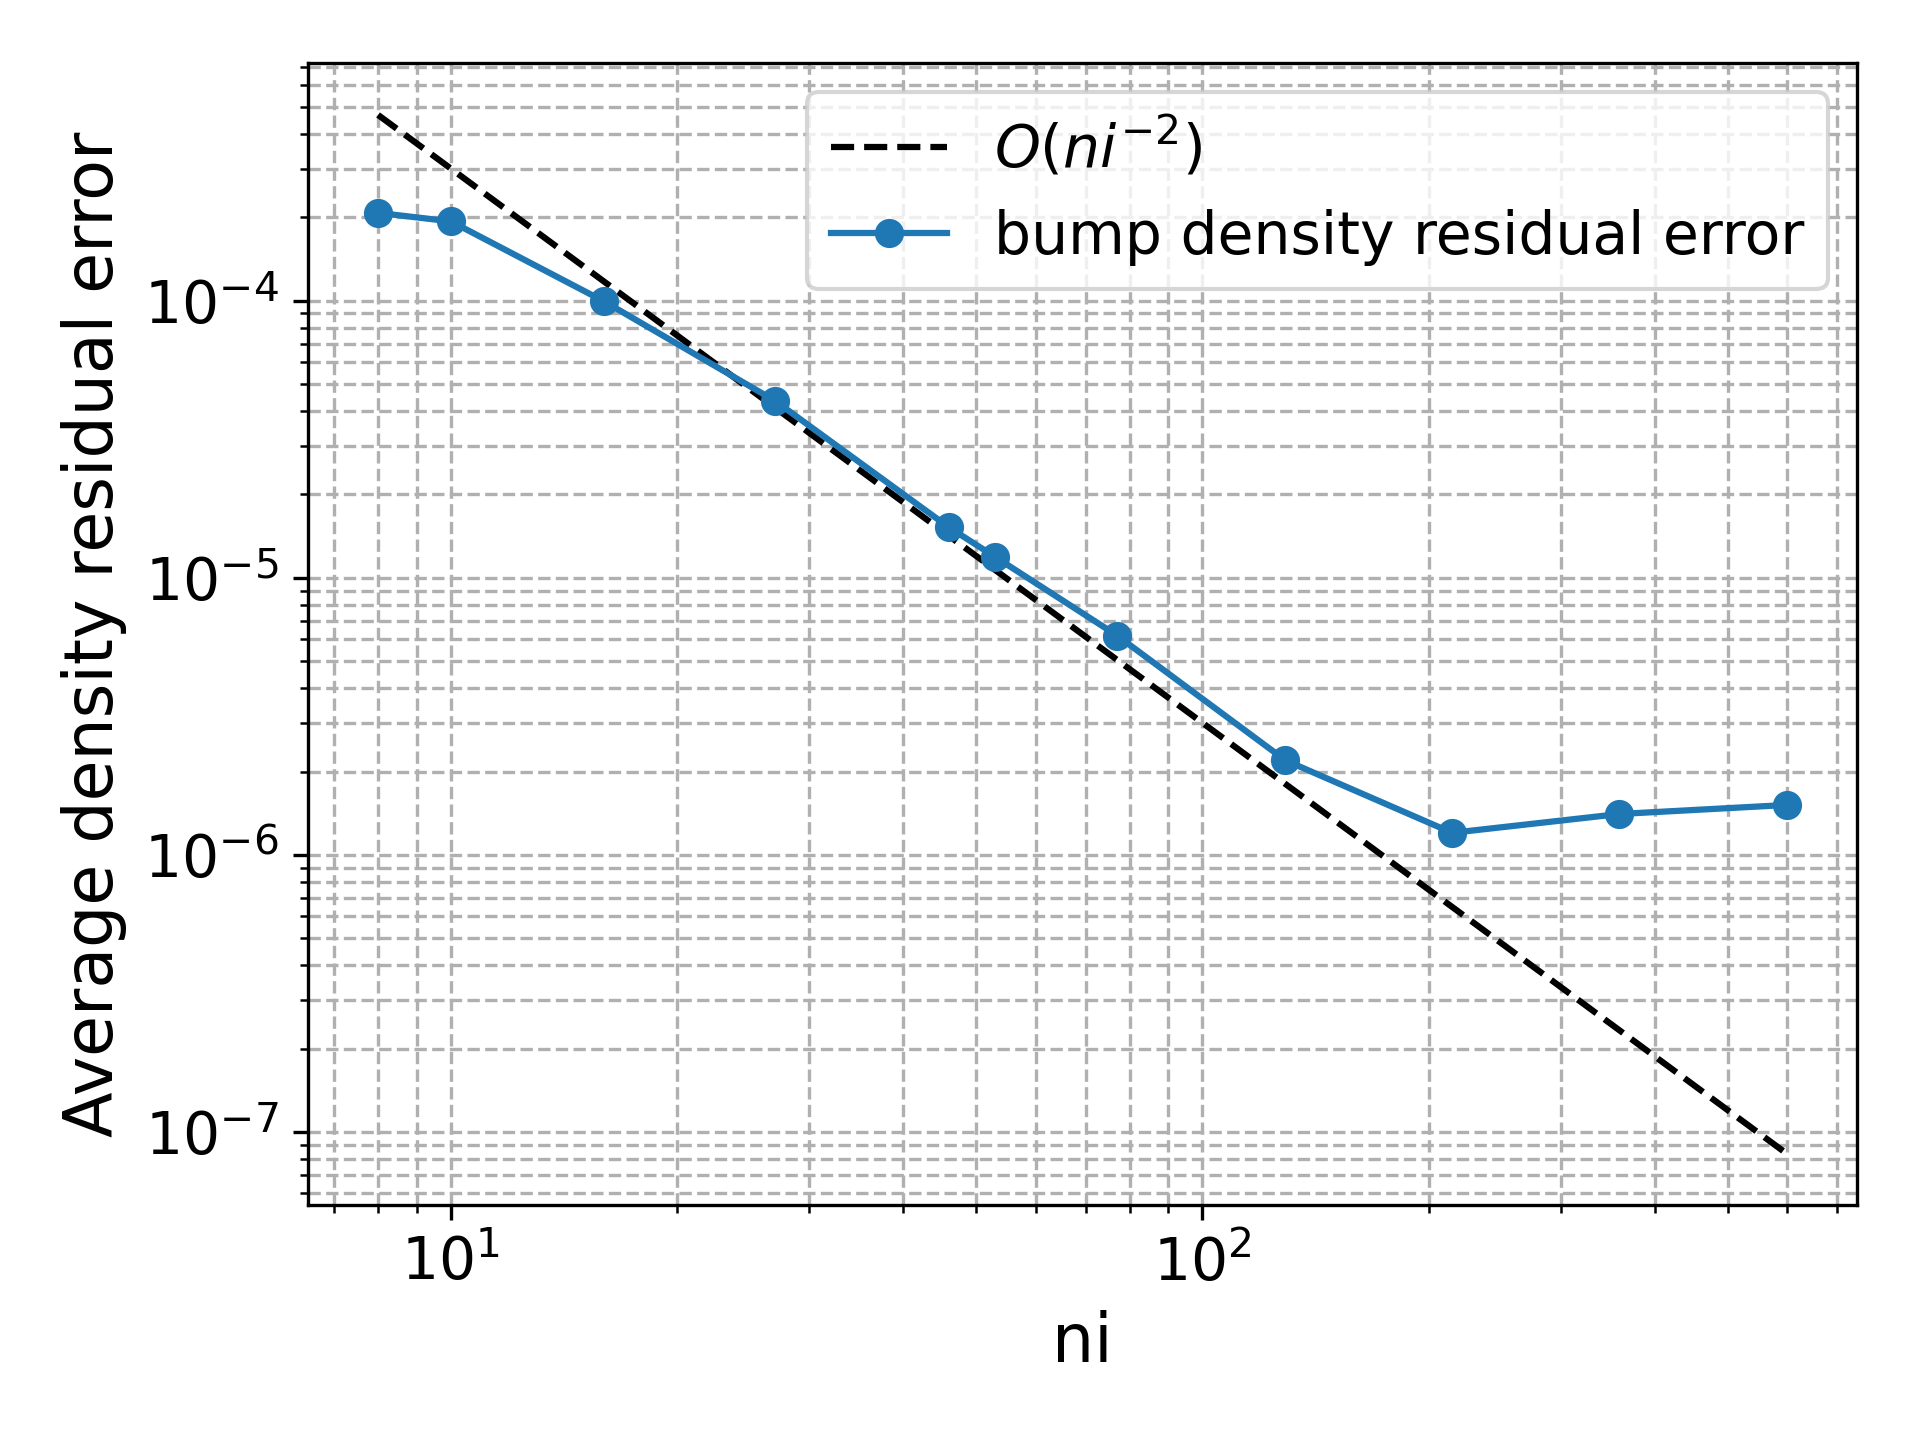
\includegraphics[width=0.8\textwidth]{figures/bump_d_avg_ni.png}
    \caption{}
    \label{fig:bump_d_avg_ni}
\end{figure}

\begin{figure}
    \centering
    \begin{subfigure}{0.49\textwidth}
        \centering
        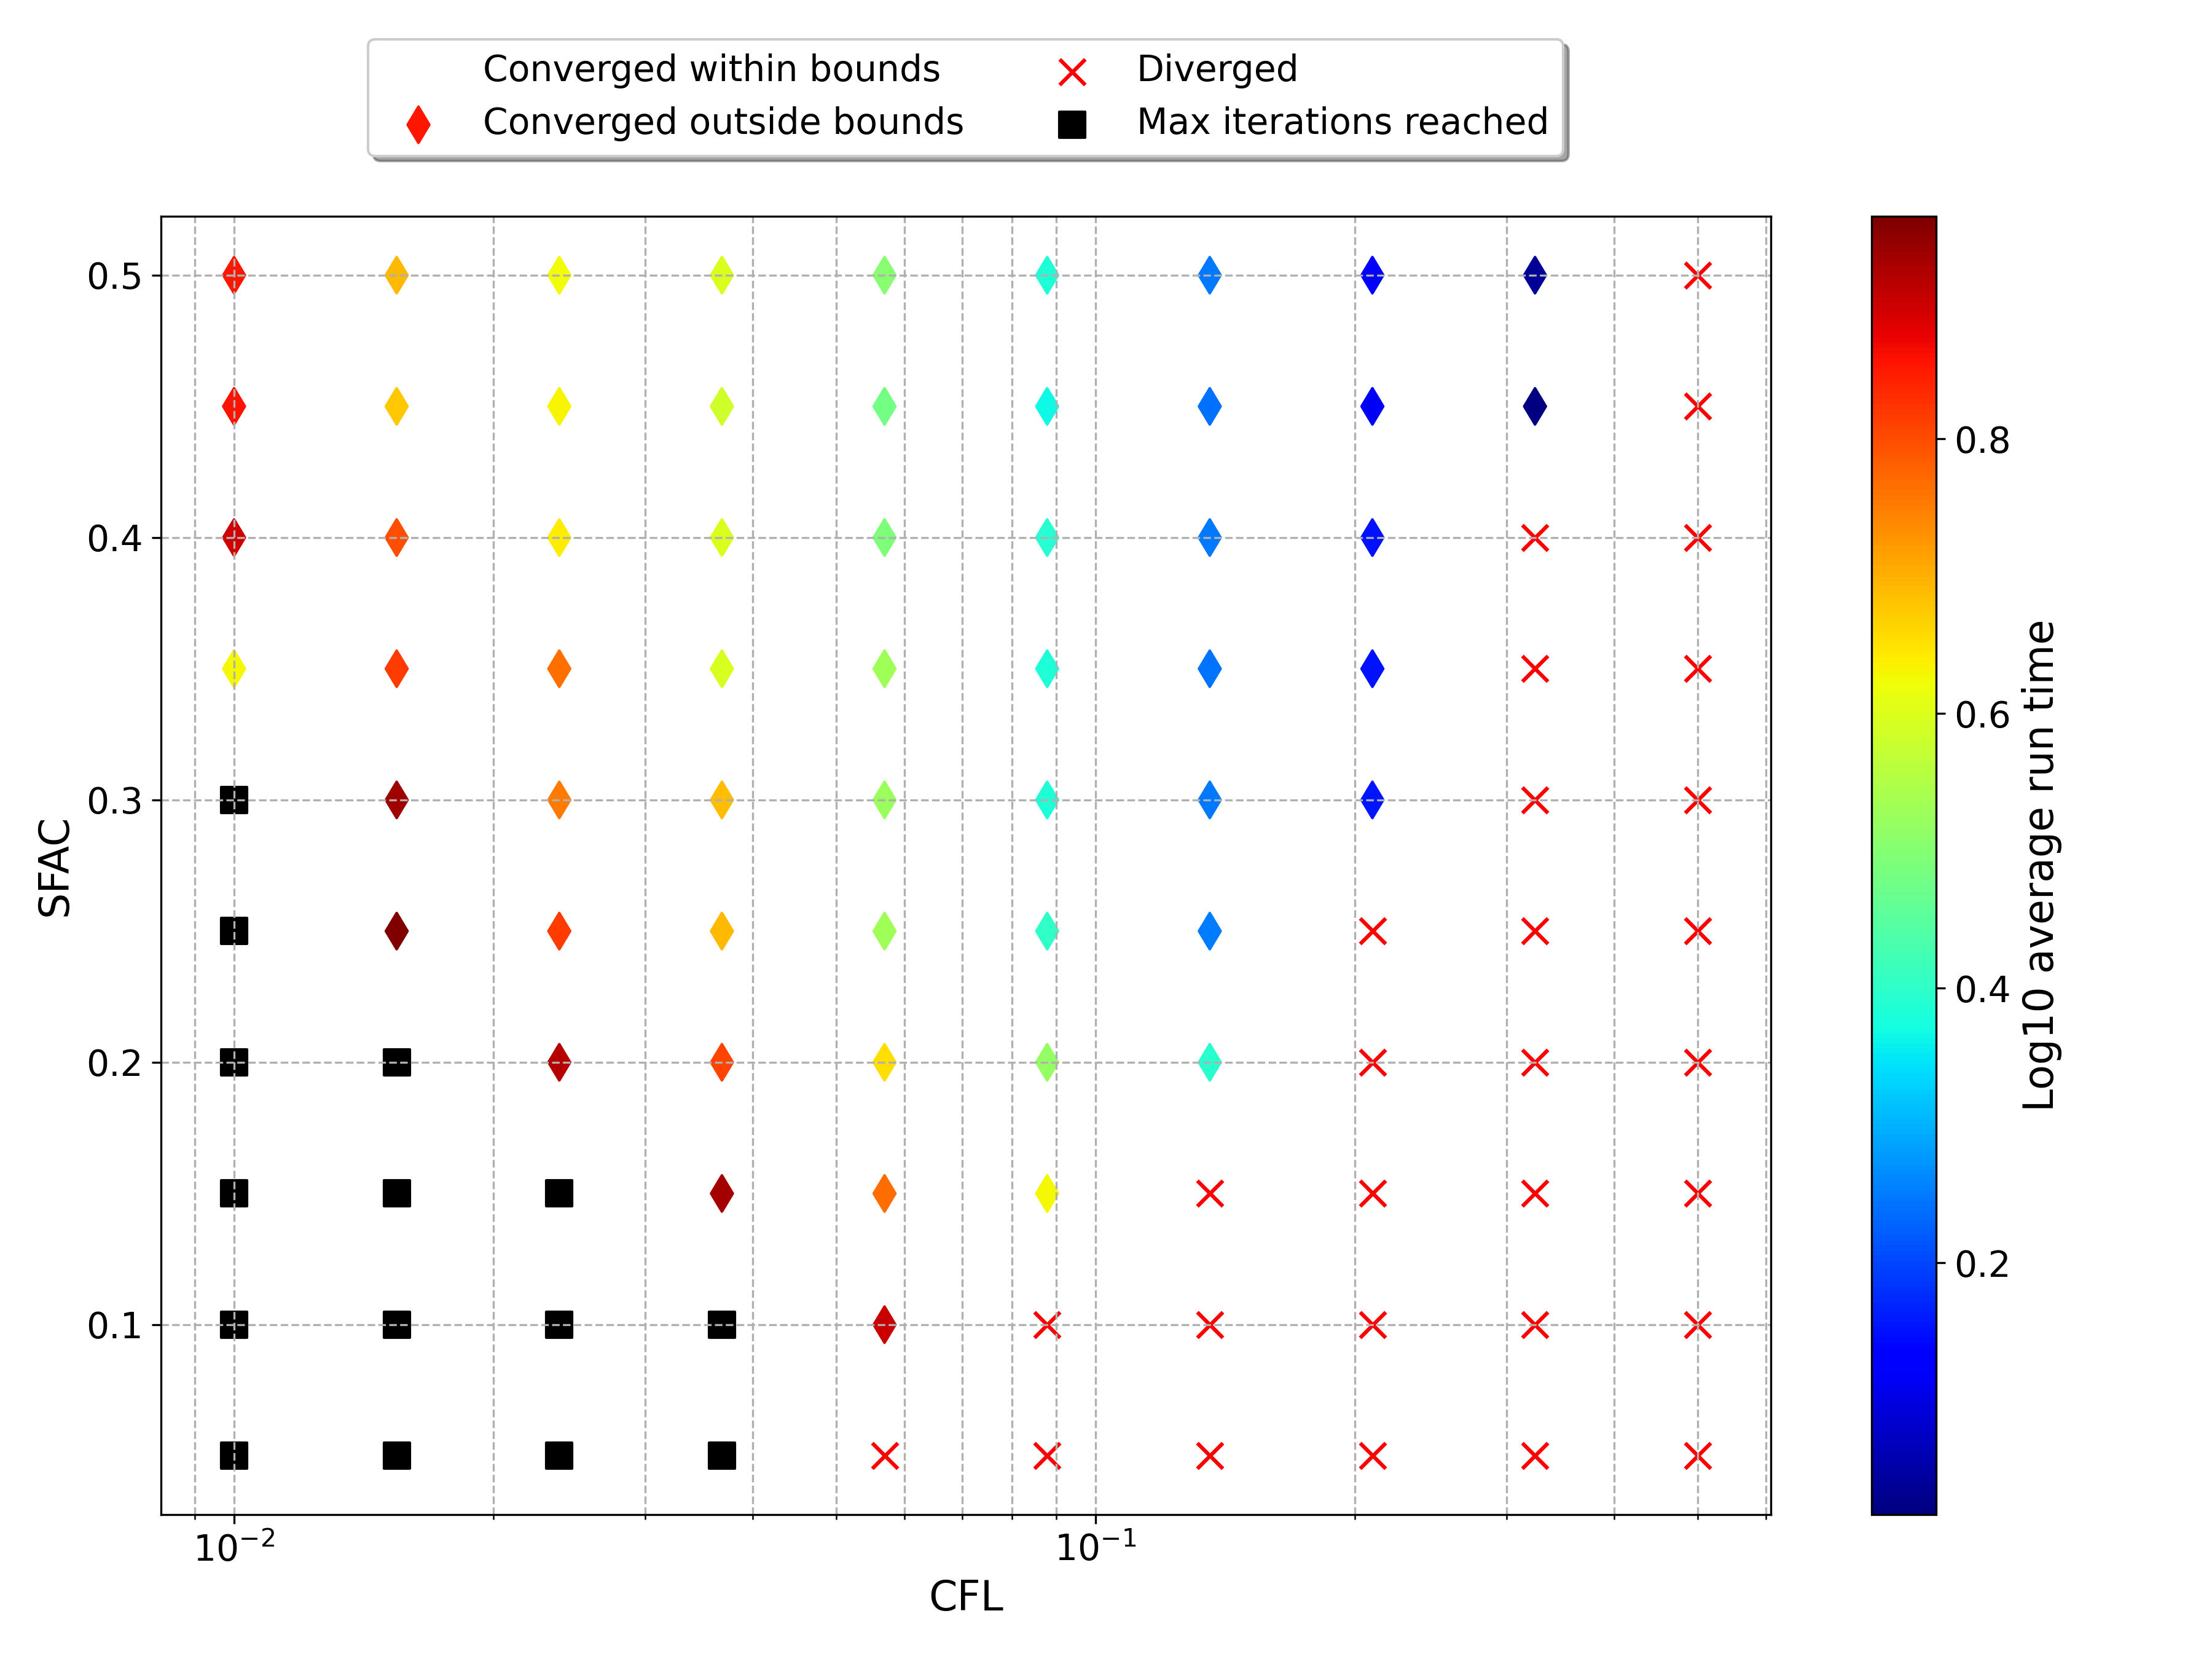
\includegraphics[width=0.99\textwidth]{figures/bump_cfl_sfac_time.png}
        \caption{}
        \label{fig:bump_time}
    \end{subfigure}
    \begin{subfigure}{0.49\textwidth}
        \centering
        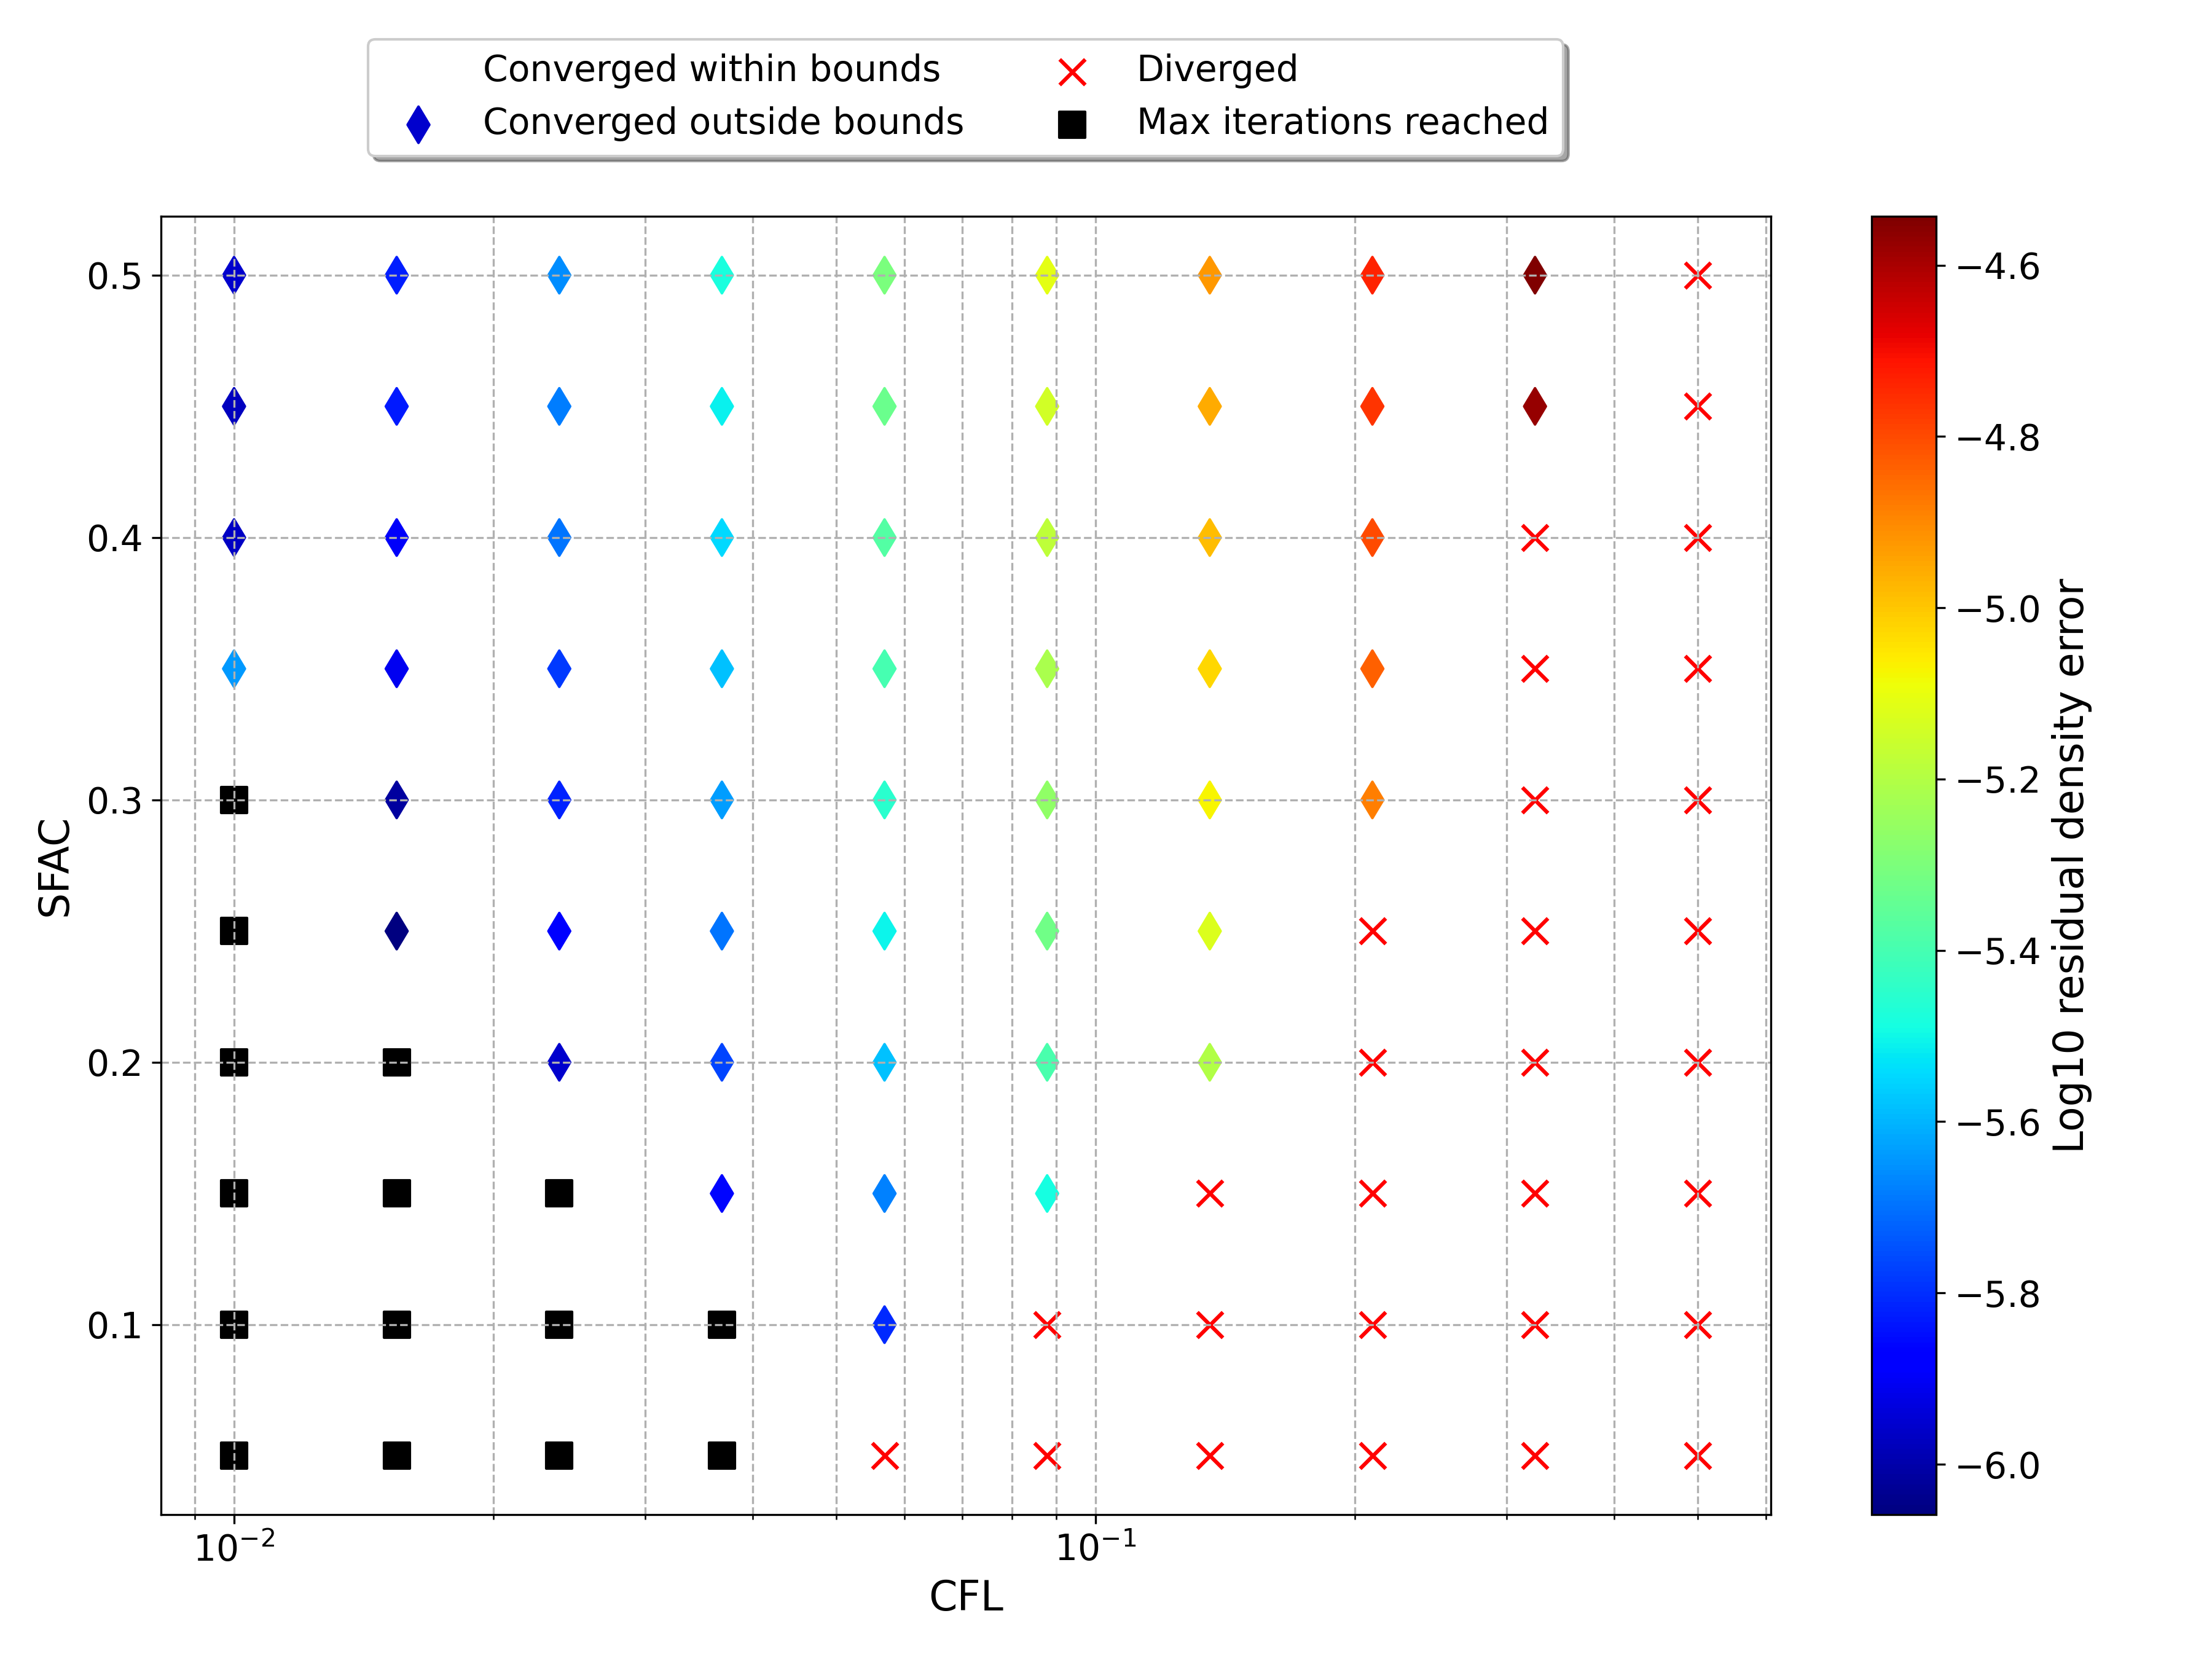
\includegraphics[width=0.99\textwidth]{figures/bump_cfl_sfac_residual.png}
        \caption{}
        \label{fig:bump_residual}
    \end{subfigure}
\end{figure}

Higher values of ni tested caused a fatal exception in chkstk.asm which indicated that the program ran out of stack space when allocating the grid arrays.
This was resolved by increasing the stack size 

\subsection{Objectives}
% set goal of what to achieve

% bibliography

\begin{thebibliography}{9}

  \bibitem{handout}
  J. V. Taylor and J. C. Massey
  \emph{GA3 Heat Exchanger Handout}
  University of Cambridge,
  2024.

\end{thebibliography}

\end{document}